\documentclass[runningheads,leqno]{llncs}

% TODO: standardise indices vs indexes
% TODO: standardise dots after equations
% TODO: rename variable maps to variable indices everywhere
% TODO: Title Case for paragraphs

\usepackage[T1]{fontenc}
\usepackage[utf8]{inputenc}
\usepackage[british]{babel}
\usepackage{newunicodechar}
\usepackage{xcolor}
\usepackage{minted}
\usepackage{amsmath,amssymb}
\usepackage{mathtools}
\usepackage{graphicx}
\usepackage{pgfplots}
\usepackage[colorlinks]{hyperref}
\usepackage{csquotes}
\usepackage[noend]{algorithm2e}
\usepackage{siunitx}
\usepackage{caption}
\usepackage{subcaption}

\bibliographystyle{splncs04}

\renewcommand\UrlFont{\color{blue}\rmfamily}
\urlstyle{rm}
\def\orcid#1{{\href{http://orcid.org/#1}{\protect\raisebox{-1.25pt}{\protect
\includegraphics{orcid.pdf}}}}}

\pgfplotsset{compat=1.18, width=8cm}
\def\showpgfcircle{\tikz[baseline=-0.7ex]\node[mark size=0.7ex]
{\pgfuseplotmark{o}};}
\def\showpgfsquare{\tikz[baseline=-0.7ex]\node[mark size=0.7ex]
{\pgfuseplotmark{square}};}

\SetKw{KwIn}{in}
\SetKw{KwLet}{let}
\SetKw{KwYield}{yield}
\SetKwInOut{Input}{Input}
\SetKwInOut{Output}{Output}
\SetKwProg{Procedure}{Procedure}{}{}

\newunicodechar{₀}{\ensuremath{_{0}}}
\newunicodechar{₁}{\ensuremath{_{1}}}
\newunicodechar{₂}{\ensuremath{_{2}}}
\newunicodechar{₃}{\ensuremath{_{3}}}
\newunicodechar{₄}{\ensuremath{_{4}}}
\newunicodechar{₅}{\ensuremath{_{5}}}
\newunicodechar{₆}{\ensuremath{_{6}}}
\newunicodechar{₇}{\ensuremath{_{7}}}
\newunicodechar{₈}{\ensuremath{_{8}}}
\newunicodechar{₉}{\ensuremath{_{9}}}
\newunicodechar{ₙ}{\ensuremath{_{n}}}
\newunicodechar{ₘ}{\ensuremath{_{m}}}
\newunicodechar{ᵢ}{\ensuremath{_{i}}}
\newunicodechar{ⱼ}{\ensuremath{_{j}}}
\newunicodechar{ₗ}{\ensuremath{_{l}}}
\newunicodechar{ₖ}{\ensuremath{_{k}}}
\newunicodechar{α}{\ensuremath{\alpha}}
\newunicodechar{σ}{\ensuremath{\sigma}}
\newunicodechar{τ}{\ensuremath{\tau}}
\newunicodechar{λ}{\ensuremath{\lambda}}
\newunicodechar{μ}{\ensuremath{\mu}}
\newunicodechar{η}{\ensuremath{\eta}}
\newunicodechar{Γ}{\ensuremath{\Gamma}}
\newunicodechar{Δ}{\ensuremath{\Delta}}
\newunicodechar{Φ}{\ensuremath{\Phi}}
\newunicodechar{Ψ}{\ensuremath{\Psi}}
\newunicodechar{Ω}{\ensuremath{\Omega}}
\newunicodechar{∈}{\ensuremath{\in}}
\newunicodechar{∉}{\ensuremath{\notin}}
\newunicodechar{≡}{\ensuremath{\equiv}}
\newunicodechar{≢}{\ensuremath{\nequiv}}
\newunicodechar{≠}{\ensuremath{\neq}}
\newunicodechar{≤}{\ensuremath{\leq}}
\newunicodechar{≥}{\ensuremath{\geq}}
\newunicodechar{≺}{\ensuremath{\prec}}
\newunicodechar{≔}{\ensuremath{\coloneq}}
\newunicodechar{∧}{\ensuremath{\land}}
\newunicodechar{∨}{\ensuremath{\lor}}
\newunicodechar{∪}{\ensuremath{\cup}}
\newunicodechar{∩}{\ensuremath{\cap}}
\newunicodechar{⊆}{\ensuremath{\subseteq}}
\newunicodechar{⋃}{\ensuremath{\bigcup}}
\newunicodechar{→}{\ensuremath{\rightarrow}}
\newunicodechar{↔}{\ensuremath{\leftrightarrow}}
\newunicodechar{↦}{\ensuremath{\mapsto}}
\newunicodechar{⊢}{\ensuremath{\vdash}}
\newunicodechar{∅}{\ensuremath{\emptyset}}
\newunicodechar{∷}{\ensuremath{\mathbin{::}}}
\newunicodechar{⇒}{\ensuremath{\Rightarrow}}
\newunicodechar{ℕ}{\ensuremath{\mathbb{N}}}
\newunicodechar{⟨}{\ensuremath{\langle}}
\newunicodechar{⟩}{\ensuremath{\rangle}}
\newunicodechar{⊤}{\ensuremath{\top}}
\newunicodechar{⊥}{\ensuremath{\bot}}
\newunicodechar{×}{\ensuremath{\times}}

\newtheorem{lem}{Lemma}

\setminted[lean4]{extrakeywords={aesop cases add aesop? intro simp simp_all only split apply on_goal next rename_i safe unsafe norm constructors forward destruct norm_num done add_aesop_rules rfl subst ext}}
\newmintinline[lean]{lean4}{bgcolor={},ignorelexererrors=true}
\newminted[leancode]{lean4}{bgcolor={},ignorelexererrors=true,fontsize=\footnotesize,autogobble}
\BeforeBeginEnvironment{leancode}{\begin{tcolorbox}}
\AfterEndEnvironment{leancode}{\end{tcolorbox}}
\usemintedstyle{xcode}

\newcommand{\para}[1]{\paragraph{\bfseries\upshape #1}}
\newcommand{\xcom}[1]{{\textcolor{cyan}{Xavier: #1}} }
\newcommand{\jcom}[1]{{\textcolor{orange}{Jannis: #1}} }

\newcommand{\Lam}[2]{\ensuremath{\lambda\, #1.\; #2}}
\newcommand{\All}[2]{\ensuremath{\forall\, #1,\; #2}}
\newcommand{\mvar}[1]{\ensuremath{{?#1}}}
\newcommand{\Prop}{\ensuremath{\mathrm{Prop}}}
\newcommand{\vars}{\ensuremath{\mathrm{svars}}}
\newcommand{\dom}{\ensuremath{\mathrm{dom}}}
\newcommand{\sub}{\ensuremath{\mathrm{sub}}}
\newcommand{\lvl}{\ensuremath{\mathrm{lvl}}}
\newcommand{\Rules}{\ensuremath{\mathcal{R}}}
\newcommand{\Hyps}{\ensuremath{\mathcal{H}}}
\newcommand{\States}{\ensuremath{\mathcal{S}}}
\newcommand{\CMatches}{\ensuremath{\mathcal{C}}}
\newcommand{\addHyp}{\ensuremath{\mathrm{addHyp}}}
\newcommand{\delHyp}{\ensuremath{\mathrm{delHyp}}}
\newcommand{\addMatch}{\ensuremath{\mathrm{addMatch}}}
\newcommand{\powerset}{\ensuremath{\mathcal{P}}}

\begin{document}

\title{Incremental Forward Reasoning for White-Box~Proof~Search}

%\titlerunning{Abbreviated paper title}
% If the paper title is too long for the running head, you can set
% an abbreviated paper title here

\author{Jannis Limperg\orcid{0000-0002-8861-5231} \and
  Xavier Généreux\orcid{0000-0003-4952-9557}}

\authorrunning{J.~Limperg and X.~Généreux}
\institute{Ludwig-Maximilians-Universität München, Munich, Germany\\
\email{\{jannis.limperg,xavier.genereux\}@lmu.de}}

\maketitle

\begin{abstract}
  Several proof assistants provide automation tactics based on tableau-style tree search, such as Isabelle's and Rocq's auto and Lean's Aesop.
  In this setting we consider \emph{forward rules}, which apply a given theorem, say, $A → B → C$, to any goal containing hypotheses $A$ and $B$, adding $C$ as a new hypothesis.
  When treated naively, such rules are tried on every goal encountered during the search, leading to repeated unifications of premises $A$ and $B$ with the hypotheses of each goal.
  We present an approach to forward rules that avoids some of this repeated work by taking advantage of similarities between successive goals.
  For each goal, we cache partial applications of forward rules in a custom data structure that enables efficient updates.
  Our technique is compatible with any search strategy and most logics.
  It has been implemented in Aesop.

  \keywords{Forward Reasoning \and Forward Chaining \and Tactics \and Interactive Theorem Proving}
\end{abstract}

\section{Introduction}

In many proof assistants, simple \enquote*{white-box} automation tactics based on tableau-style tree search play a substantial role in practice: Isabelle's~\cite{Isabelle} and Rocq's~\cite{Coq} auto~\cite{IsabelleAuto}, ACL2's \enquote{waterfall}~\cite{ACL2}, various PVS~\cite{PVS-tutorial,PVS} tactics, Lean's~\cite{Lean4} Aesop~\cite{Aesop}, etc.
These tactics operate on \emph{goals} $Γ ⊢ A$, where the \emph{context} $Γ$ is a list of assumptions and $A$ is the proposition to be proved.
Faced with an initial goal, the tactics try various user-specified \emph{rules}, which correspond to admissible inferences in the prover's logic.
A successful rule reduces the current goal to zero or more subgoals, which are solved recursively until either a full proof is found or no rule applies to any open goal or the search times out.
A typical rule is the $∧$-introduction lemma $A → B → A ∧ B$, which, when applied backwards, reduces a goal $Γ ⊢ A ∧ B$ to subgoals $Γ ⊢ A$ and $Γ ⊢ B$.

In addition to such \emph{backwards rules}, most search tactics can also use arbitrary tactics as rules.
For example, Aesop uses the cases tactic on disjunctive hypotheses, splitting goals of the form $Γ,\, h : A ∨ B ⊢ C$ into subgoals $Γ,\, h : A ⊢ C$ and $Γ,\, h : B ⊢ C$.
Tactics implement arbitrary inferences; in particular, they can remove any hypothesis and add any provable proposition as a new hypothesis.

ACL2, PVS and Aesop additionally provide special support for \emph{forward reasoning}, also known as \emph{forward chaining}, in the form of \emph{forward rules}.
Given, for example, the transitivity lemma $\All{x~y~z}{x < y → y < z → x < z}$, a forward rule run on the goal $h₁ : a < b,\, h₂ : b < c ⊢ A$ produces the single subgoal $h₁ : a < b,\, h₂ : b < c,\, h₃ : a < c ⊢ A$.
Hence forward rules can be used to establish additional facts that may be relevant for other rules.
For example, the Aeneas project~\cite{Aeneas} uses Aesop's forward rules in its proof automation to establish facts that are later used by an arithmetic decision procedure.

Until recently, Aesop used what we call the \emph{naive algorithm} to apply forward rules.
When a forward rule was run on a goal, the rule would search the goal's context for all combinations of hypotheses satisfying its premises.
This method is simple but involves much repeated work because in practice, contexts encountered during the search tend to be similar.
For example, the ∧-introduction rule, when run on $Γ ⊢ A ∧ B$, produces subgoals $Γ ⊢ A$ and $Γ ⊢ B$, so the naive algorithm runs the same forward rules on the same context $Γ$ three times.
More generally, any backwards rule leaves the context unchanged, and many rules that change the context do so only in limited ways.

In this paper, we present an alternative way to apply forward rules that addresses this issue.
The central idea is to remember, for each goal $Γ ⊢ A$, which forward rules can be partially applied to which sets of hypotheses.
When a non-forward rule then generates subgoals $Δ₁ ⊢ A₁$, \dots, $Δₙ ⊢ Aₙ$, the new contexts $Δᵢ$ are likely similar to $Γ$.
Hence it is generally cheaper (and often much cheaper) to start with the partial matches for $Γ$ and update them for each of the $Δᵢ$.
The update first deletes partial matches that include hypotheses no longer present in $Δᵢ$.
Afterwards it adds new partial matches for the hypotheses that are new in $Δᵢ$, extending the existing partial matches for a rule if the new hypothesis is compatible with them.
Whenever this process produces a full match---i.e., all premises of a forward rule are satisfied by a set of hypothesis in $Δᵢ$---the rule is applied and adds a corresponding new hypothesis to $Δᵢ$.

Our main contribution is a data structure, the \emph{forward state}, that organises the partial matches so that updates can be done efficiently.
In addition to this \emph{incrementality}, the forward state satisfies two other desiderata:
\begin{itemize}
  \item It is \emph{persistent}, i.e.\ forward states for parent and child goals share much of their structure.
        This is desirable since Aesop supports search strategies other than depth-first search and must therefore keep all goals encountered during the search, along with their forward states, in memory.
  \item It reduces the number of \emph{unifications} performed when matching hypotheses against rule premises.
        In dependent type theory, unification happens up to definitional equality, which makes it expensive.
        We therefore want to avoid redundant unifications.
\end{itemize}

Our evaluation (Sec.~\ref{sec:evaluation}) shows that this new implementation of forward reasoning in Aesop substantially outperforms the previous, naive implementation on synthetic benchmarks.
The implementation, benchmarks and evaluation data are available in a supplement to this paper~\cite{supplement} and the new implementation is already available in the newest version of Aesop.

\section{Preliminaries}

We first introduce some terminology for matches and for forward rules (which we identify with their underlying lemmas).
We use dependent type theory as a foundation, but our technique generalises to other logics.

Given a lemma $\All{(x₁ : A₁) \dots (xₙ : Aₙ)}{B}$, the $xᵢ$ are \emph{premises} and $B$ is the lemma's \emph{conclusion}.
The type $Aᵢ$ of the $i$th premise may depend on (i.e., refer to) any premise $xⱼ$ with $j < i$.
Implication $A → B$ is an abbreviation for $\All{x : A}{B}$ where $B$ does not depend on $x$.
Propositions are (certain) types, and we do not distinguish between the two concepts.

Using somewhat non-standard terminology, we call premises on which a later premise depends \emph{variables}.
These are typically terms of non-propositional types, e.g.\ natural numbers or lists.
The non-variable premises, whose types are typically propositions, are called \emph{slots}.
For example, the lemma $\All{(x~y~z : ℕ)}{x < y → y < z → x < z}$ has variables $x, y, z$ and slots of types $x < y$ and $y < z$.
If more than two premises depend on a variable (e.g.\ $y$), the variable is \emph{shared}.
Note that premises on which only the conclusion depends are not considered variables.

If a lemma has $n$ slots, each slot is assigned a unique number between $1$ and $n$, and we identify slots with their numbers.
For now, we assume that the slots are numbered consecutively, so in the example above slot~1 has type $x < y$ and slot~2 has type $y < z$.
The \emph{shared variables of slot $i$}, $\vars(i)$, are those variables that appear in the type of $i$ and also in at least one type of a slot $j < i$.

If $h : C$ is a hypothesis and $C$ matches the type $A$ of slot $i$, we say that $h$ \emph{matches} $i$.
Matching induces a substitution $σ$ such that $A[σ]$ is definitionally equal to $C$; we define $\sub_{i}(h) ≔ σ$.
What exactly \enquote{matching} means is discussed in Sec.~\ref{sec:implementation}.

A \textit{match} $m$ for a given rule $r$ with $n$ slots is a list containing at least one and at most $n$ hypotheses.
We interpret $m$ as a partial map from slots of $r$ to hypotheses, so $\dom(m) = \{i \mid 1 ≤ i ≤ |m| \}$ and for each slot $i ∈ \dom(m)$, $m(i)$ is the hypothesis assigned to $i$.
A match $m$ must additionally satisfy the following requirements:
\begin{enumerate}
  \item\label{cond:match:matches} For each slot $i ∈ \dom(m)$, the hypothesis $m(i)$ matches $i$.

  \item\label{cond:match:compat} For all slots $i,j ∈ \dom(m)$, the substitutions $\sub_{i}(m(i))$ and $\sub_{j}(m(j))$ are \emph{compatible}.
        This means that the substitutions agree on all common variables, i.e.\ for each variable $x ∈ \dom(\sub_{i}(m(i))) ∩ \dom(\sub_{j}(m(j)))$ we have $\sub_{i}(m(i))(x) = \sub_{j}(m(j))(x)$.
\end{enumerate}
The \emph{substitution of a match $m$}, $\sub(m)$, is the union of the substitutions induced by the hypotheses in $m$, i.e. $\sub(m) ≔ ⋃_{i ∈ \dom(m)}\sub_{i}(m(i))$.
This is well defined by requirement~\ref{cond:match:compat}.
The \textit{level of a match $m$}, $\lvl(m)$, is the length of $m$.
A match for rule $r$ is \textit{complete} if $i ∈ \dom(M)$ for every slot $i$ of $r$, and \emph{partial} otherwise.

A partial match $m$ for rule $r$ corresponds to a partial application of the rule to the terms given in $\sub(M)$.
The application is type-correct by requirements~\ref{cond:match:matches} and~\ref{cond:match:compat}.
If $m$ is complete, then $\sub(m)$ contains a term for every slot and every variable---hence for every premise---of $r$ and we have a full application.

Note that matches represent only those partial applications where arguments are added without gaps.
Hence for a rule $r : A → B → C → D$, the applications $r~a~\_ : B \to D$ and $r~a~b : D$ for some $a : A$ and $b : B$ correspond to matches, but not $r~\_~b : A \to D$.
This prevents us from constructing $r~a~b$ in two different but ultimately redundant ways.
The term orders used in various saturation calculi serve a similar function.

\section{Naive Forward Reasoning}%
\label{sec:naive}

Before this work, Aesop used what we call \emph{naive forward reasoning}~\cite{Aesop}.
This approach treats forward rules essentially like any other Aesop rule.
Hence, when Aesop selects a forward rule $r$ with $n$ slots of types $A₁, \dots, Aₙ$ as the highest-priority rule currently applicable to a goal $Γ ⊢ T$, we look for all complete matches for $r$ in $Γ$, using an approach reminiscent of backtracking subsumption algorithms.

More specifically, we first match the type of the last slot, $Aₙ$, with each hypothesis $h : B$ (using a discrimination tree index to quickly determine potentially matching hypotheses).
If successful, this results in a substitution $σ₁$ containing all variables that occur in $Aₙ$.
We then match $A_{ₙ-1}[σ₁]$ against the type of each hypothesis in the context, yielding a substitution $σ₂$, and proceed with $A_{ₙ-2}[σ₂]$, etc., until we obtain a complete match for $r$.
If a premise $A_{ₙ-i}[σᵢ]$ does not match any hypothesis type, we backtrack and consider other potential matching hypotheses for $A_{ₙ-i+1}$.
These may lead to a different substitution $τ$ and therefore to different matching hypotheses for $A_{ₙ-i}[τ]$.
For each complete match $m$ with substitution $σ$ found during this process, we add a new hypothesis of type $B[σ]$, where $B$ is the conclusion of $r$.

This approach is efficient when the last slot of a rule is not present in the context since the rule is then excluded by indexing and never run.
Otherwise, we match large numbers of premises and hypotheses against each other, though this process could likely be sped up heuristically~\cite{TammetSubsumption}.
Moreover, the whole process is repeated when we proceed to another goal with a similar context.
In particular, the contexts of subgoals produced by whatever rule is eventually applied to the current goal are likely to be similar to the current context, but the naive algorithm does not exploit these similarities.

\section{Incremental Forward Reasoning}%
\label{sec:incremental}

With the weaknesses of the naive approach in mind, we introduce an incremental, stateful solution to the problem of finding complete matches.
The main idea is to store, for each goal $Γ ⊢ A$, the partial matches implied by the hypotheses in $Γ$, and to reuse these partial matches for subgoals $Δ ⊢ B$.
This rests on the assumption that $Δ$ is likely similar to $Γ$ in practice, and that it is therefore cheaper to update the partial matches for $Γ$ than to compute those of $Δ$ from scratch.
Our main contribution is a data structure, the \emph{forward state}, that allows us to perform these updates efficiently.

\para{Forward States.}
We associate with each goal in Aesop's search tree a forward state that reflects the goal's context.
Let $\States$ be the set of forward states, $\Hyps$ the set of hypotheses, $\Rules$ the set of rules, $\CMatches$ the set of complete matches and $\powerset(X)$ the powerset of $X$.
The forward state's interface then consists of two functions
\begin{equation*}
  \addHyp : \States → \Hyps → \States × \powerset(\Rules × \CMatches) \qquad \delHyp : \States → \Hyps → \States
\end{equation*}
The $\addHyp$ function adds a hypothesis to the forward state.
Hence, if $s$ is the forward state corresponding to context $Γ$ and $\addHyp(s,\, h : T) = (s', C)$, then $s'$ is the forward state corresponding to $Γ,\, h : T$.
Similarly, if $s$ is the forward state corresponding to $Γ,\, h : T$, then $\delHyp(s,\, h : T)$ is the forward state corresponding to $Γ$.
The second output of $\addHyp$, $C$, is a set of pairs $(r, m)$ where $r$ is a rule and $m$ is a complete match for $r$.
These are the matches that were completed by adding $h : T$.

When Aesop is run on an initial goal with context $h₁ : T₁, \dots, hₙ : Tₙ$, the forward state for it is built by starting with an empty state and applying $\addHyp$ to each hypothesis $hᵢ$.
Afterwards, whenever an Aesop rule is run on a goal with context $Γ$, producing subgoals with contexts $Δ₁, \dots, Δₙ$, we derive the forward state for each subgoal context $Δⱼ$ from the forward state for $Γ$, in two steps:
\begin{enumerate}
  \item Apply $\delHyp$ once for each hypothesis that was deleted, i.e.\ that appears in $Γ$ but not in $Δⱼ$.
  \item Apply $\addHyp$ once for each hypothesis that was added, i.e.\ that appears in $Δⱼ$ but not in $Γ$.
\end{enumerate}
Changes to a hypothesis (e.g.\ a change of its type) are treated as a deletion followed by an addition.

\para{Rule States.}
Partial matches are specific to each rule, so the forward state naturally decomposes into a set of \emph{rule states}, one per rule.
Given a goal $Γ ⊢ A$ and a rule $r$, the rule state for $r$ contains exactly the partial matches of $r$ in context $Γ$.
A rule state supports $\addHyp$ and $\delHyp$ methods analogous to those on forward states.
Adding a hypothesis to a forward state then amounts to adding it to each rule state (which may yield new complete matches for the rule); deleting a hypothesis amounts to deleting it from each rule state.
We initially focus on how to add hypotheses, since this question motivates much of the design of the rule state data structure.

When a hypothesis is added to a rule state, two things can happen.
First, the hypothesis may allow us to extend partial matches already present in the state.
For instance, consider the rule $r : \All{x}{P~x → Q~x → R~x → S~x}$ and a rule state containing the partial match $[h₁]$, which assigns some hypothesis $h₁ : P~a$ to the first slot of type $P~x$.
Adding a new hypothesis $h₂ : Q~a$ to this rule state means that we should add to the state the extended match $[h₁, h₂]$.

Second, adding a match may trigger the insertion of further matches.
Suppose that before adding $h₁$ and $h₂$, we had already added a hypothesis $h₀ : R~a$ to the rule state.
Once the partial match $[h₁, h₂]$ arrives, we should recognise that it can be extended with $h₀$ to obtain the (complete) match $[h₁, h₂, h₀]$.

\para{Variable Indices.}
Extending the matches above was possible only because all hypotheses are compatible on the shared variable $x$, i.e.\ they all instantiate $x$ with the same term $a$.
In general, to extend a match $m$ with a hypothesis $h : T$ at slot $i$, we need to ensure that the substitution of $m$, $\sub(m)$, is compatible with the substitution of $h$, $\sub_{i}(h)$.

The rule state therefore uses two \emph{variable indices} $H$ and $M$ to index hypotheses and matches by their instantiations for shared variables, allowing us to quickly determine compatible pairs of matches and hypotheses.
We could use a substitution tree~\cite{SubstitutionTrees}, but our custom data structure is simpler and perhaps more efficient.
The \emph{hypothesis index} $H$ maps each triple $(x, i, t)$ (where $i > 1$ is a slot, $x ∈ \vars(i)$ a variable and $t$ a term) to the set of hypotheses $h$ added to the rule state such that $h$ matches $i$ and $\sub_{i}(h)(x) = t$.
In other words, $H$ indexes the known hypotheses by the slots they match and the instantiations of shared variables.
Note that hypotheses matching slot $1$ are not stored since they can never extend a match.

Similarly, the \emph{match index} $M$ maps each triple $(x, i, t)$ to the set of partial matches $m$ (that can be derived from the hypotheses added to the rule state) such that $i = \lvl(m) $, $x ∈ \vars(i + 1)$ and $\sub(m)(x) = t$.
Matches for the maximal slot are not stored because, being complete, they never need to be extended.
We write $M_{x}(i, t)$ instead of $M(x, i, t)$ and $H_{x}(i, t)$ instead of $H(x, i, t)$.

Given a hypothesis $h : T$ that matches slot $i > 1$ with substitution $σ = \sub_{i}(h)$, the partial matches that can be extended by $h$ are those in slot $i - 1$ whose substitutions are compatible with $σ$ on the variables $\vars(i)$ (i.e., the variables shared between $i$ and any earlier slot).
Assuming for the moment that $\vars(i)$ is nonempty for all slots $i > 1$, these matches are
\[
  \bigcap_{x \in \vars(i)} M_{x}(i-1, σ(x))
\]
Similarly, given a partial match $m$ at level $i$ with substitution $σ = \sub(m)$, the hypotheses that could extend $m$ are
\[
  \bigcap_{x \in \vars(i+1)} H_{x}(i+1, σ(x))
\]
The number of shared variables tends to be small in practice, so these intersections can be computed efficiently.

From these observations we can directly derive two procedures for adding hypotheses and matches to the rule state.
The procedures maintain the invariants of the variable indices while reporting any complete matches discovered during this process.
Specifically, if a rule state for a rule $r$ represents the context $Γ$---i.e., it contains the hypotheses of $Γ$ and all partial matches of $r$ that can be derived from them---then the rule state obtained from $\addHyp(h : T)$ represents $Γ,\, h : T$.

\begin{algorithm}
  \Input{A hypothesis $h : T$}
  \Output{All complete matches of $r$ in context $Γ,\, h : T$ that contain $h$}
  \BlankLine
  \Procedure{$\mathrm{addHyp}(h : T)$}{
    \For{all slots $i$ of $r$ such that $h$ matches $i$}{
      \eIf{$i = 1$}{
        $\mathrm{addMatch}([h])$
      }{
        \KwLet $σ ≔ \sub_{i}(h)$ \\
        \For{$x$ \KwIn $\vars(i)$}{
          Insert $h$ into the set $H_{x}(i, σ(x))$
        }
        \KwLet $\mathit{ms} ≔ \bigcap_{x \in \vars(i)} M_{x}(i-1, σ(x))$ \\
        $\mathit{completeMs} \gets ∅$ \\
        \For{$m$ \KwIn $\mathit{ms}$}{
          $\mathit{completeMs} \gets \mathit{completeMs} ∪ \mathrm{addMatch}(m \mathbin{++} [h])$
        }
        \Return{$\mathit{completeMs}$}
      }
    }
  }
  \BlankLine % without these, the caption is not offset properly
  \BlankLine
  \caption{Add a hypothesis to the rule state for a rule $r$ and context $Γ$}%
  \label{alg:addhyp}
\end{algorithm}

The rule state's $\addHyp$ method (Algorithm~\ref{alg:addhyp}) adds a hypothesis $h : T$ matching slot $i$ to the rule state.
(If a hypothesis matches multiple slots, $\addHyp$ is called multiple times.)
For $i = 1$, we add the singleton match $[h]$ to the rule state.
For $i > 1$, we first insert $h$ into the hypothesis index $H$.
Then we query the match index $M$ for matches that can be extended by $h$ and add the extended matches to the rule state.
While adding matches, we may discover new complete matches, which are collected and returned.

\begin{algorithm}
  \Input{A partial match $m$ of $r$ at level $i$ with substitution $σ$}
  \Output{A set of complete matches of $r$}
  \BlankLine
  \Procedure{$\mathrm{addMatch}(m)$}{
    \eIf{$i$ is complete}{
      \Return{$\{m\}$}
    }{
      \For{$x$ \KwIn $\vars(i + 1)$}{
        Insert $m$ into the set $M_{x}(i, σ(x))$
      }
      \KwLet $\mathit{hs} ≔ \bigcap_{x \in \vars(i + 1)} H_{x}(i + 1, σ(x))$ \\
      $\mathit{completeMs} \gets ∅$ \\
      \For{$h$ \KwIn $\mathit{hs}$}{
        $\mathit{completeMs} \gets \mathit{completeMs} ∪ \mathrm{addMatch}(m \mathbin{++} [h])$
      }
      \Return{$\mathit{completeMs}$}
    }
  }
  \BlankLine % without these, the caption is not offset properly
  \BlankLine
  \caption{Add a match to the rule state for a rule $r$}%
  \label{alg:addmatch}
\end{algorithm}

The rule state's $\addMatch$ method (Algorithm~\ref{alg:addmatch}) adds a match $m$ with level $i = \lvl(m)$ to the rule state.
If $m$ is already complete, it is returned.
Otherwise $m$ is inserted into $M$ and we query $H$ for hypotheses that can extend $m$.
Any extended matches thus produced are added to the rule state recursively.

\para{Variable Clusters.}
We have so far only considered rules where for each slot $i > 1$, the set of shared variables $\vars(i)$ is nonempty, i.e.\ each slot shares at least one variable with at least one of the previous slots.
However, there are also rules such as $\All{x~y}{P~x → Q~y → R~x~y}$, where slot~2 ($Q~y$) shares no variables with slot~1 ($P~x$).
In this case, any match at level 1 can be extended with any hypothesis at level 2, since the two slots are independent.

To account for this fact, we partition the set of premises of each rule into maximal subsets of premises connected by shared variables, called \emph{variable clusters}, using the same construction as Aesop's \emph{metavariable clusters}~\cite{Aesop}.
The variable clusters share no variables with each other, so each can be treated as a separate rule with its own rule state.
Finding a complete match for a rule then amounts to finding one complete match for each of its clusters.
The slots within each cluster can be ordered to ensure that each slot shares at least one variable with the previous slots, satisfying our assumption.

\para{Deletion.}
When a hypothesis $h$ is removed from a goal's context, we must update the forward state accordingly.
This means deleting $h$ from any rule state to which it was previously added, i.e.\ from any rule state for a rule $r$ with a slot $i$ matching $h$.
To facilitate deletion, we cache this information when $h$ is added to the rule state.
When $h$ is deleted, we can then efficiently determine the relevant rule states and delete $h$ from the hypothesis index $H$ at slot $i$ and from the match index $M$ at all slots $j ≥ i$.

\para{Example 1.}
As a first example, consider a rule state for the transitivity rule $r₁ : \All{x~y~z}{x ≤ y → y ≤ z → x ≤ z}$ to which we add, in order, the hypotheses
$h₁ : b ≤ c$ and $h₂ : a ≤ b$.
The rule has two slots of types $x ≤ y$ and $y ≤ z$ which share the variable $y$.

The hypothesis $h₁ : b ≤ c$ unifies with both slots, so we run Algorithm~\ref{alg:addhyp} twice.
For slot 1, unification yields the substitution $\{x ↦ b, y ↦ c\}$.
Since this is the first slot, Algorithm~\ref{alg:addmatch} inserts the new partial match $[h₁]$ into the set $M_{y}(1, c)$.
This match cannot be extended since the hypothesis index $H$ does not contain a hypothesis for slot 2.

For slot~2, unification yields the substitution $σ ≔ \{y ↦ b, z ↦ c\}$, so we insert $h₁$ into $H_{y}(2, b)$.
No matches at level~1 can be extended by $h₁$ since
\[
  \bigcap_{x \in \vars(2)} M_{x}(1, σ(x)) = M_{y}(1, b) = \emptyset
\]
At this point, $H$ and $M$ are in state~\eqref{eq:example1:state1}, shown below.

\begin{center}
  \begin{minipage}{0.43\textwidth}
    \begin{center}
      \begin{align}\label{eq:example1:state1}
        H_y\colon
        \begin{tikzpicture}[baseline={([yshift=-.5ex]current bounding box.center)}, outer sep=auto, level distance=4em, scale=0.5]
          \node at (0,0) {2}
            child {node {$b$}
              child {node {$\{h₁\}$}}};
        \end{tikzpicture}
        && M_y\colon
        \begin{tikzpicture}[baseline={([yshift=-.5ex]current bounding box.center)}, outer sep=auto, level distance=4em, scale=0.5]
          \node at (0, 0) {1}
            child {node {$c$}
              child {node {$\{[h₁]\}$}}};
        \end{tikzpicture}
      \end{align}
    \end{center}
  \end{minipage}
  \begin{minipage}{0.56\textwidth}
    \begin{center}
      \begin{align}\label{eq:example1:state2}
        H_y\colon
        \begin{tikzpicture}[baseline={([yshift=-.5ex]current bounding box.center)}, level distance=4em, scale=0.5]
          \node at (0,0) {2}
            child {node[xshift=-2] {$b$}
              child {node {$\{h₁\}$}}}
            child {node[xshift=2] {$a$}
              child {node {$\{h₂\}$}}};
        \end{tikzpicture}
        && M_y\colon
        \begin{tikzpicture}[baseline={([yshift=-.5ex]current bounding box.center)}, outer sep=auto, level distance=4em, scale=0.5]
          \node at (-1, 0) {1}
            child {node[xshift=-4] {$c$}
              child {node {$\{[h₁]\}$}}}
            child {node[xshift=4] {$b$}
              child {node {$\{[h₂]\}$}}};
        \end{tikzpicture}
      \end{align}
    \end{center}
  \end{minipage}
\end{center}

Now we add $h₂ : a ≤ b$, which again unifies with both slots.
For slot~1, $\sub₁(h₂)(y) = b$, so we add the match $[h₂]$ to $M_{y}(1, b)$.
We then check for hypotheses in slot~2 that also instantiate $y$ with $b$, and indeed we find $H_{y}(2, b) = \{h₁\}$.
Hence we return the complete match $[h₂, h₁]$, which induces a new hypothesis $h₃ : a ≤ c$ to be added later.
For slot~2, we add $h₂$ to $H_{y}(2, a)$.
There are no compatible matches at level~1 so we are done with $h₂$, yielding the final rule state~\eqref{eq:example1:state2}.

\para{Example 2.}
We now consider a rule $r₂ : \All{x~y}{A~x~y → B~x~y → C~x~y}$ with multiple shared variables.
We add hypotheses $h₁ : B~a~a$, $h₂ : A~a~b$ and $h₃ : B~a~b$ to the rule state of $r₂$, starting with $h₁$, which is added to $H$ with slot~2.
There are no matches yet, so there is nothing to extend.
We then add $h_2 : A~a~b$, which initially generates a match $m = [h₂]$ that is added to $M$, yielding the following rule state:
\begin{align*}
  H_x\colon
  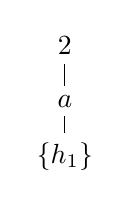
\begin{tikzpicture}[baseline={([yshift=-.5ex]current bounding box.center)},outer sep=auto, level distance=4em, scale=0.50]
    \node at (0, 0) {2}
      child {node {$a$}
        child {node {$\{h_1\}$}}};
  \end{tikzpicture}
  &&
  H_y\colon
  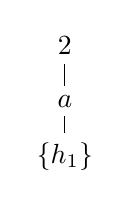
\begin{tikzpicture}[baseline={([yshift=-.5ex]current bounding box.center)},outer sep=auto, level distance=4em, scale=0.50]
    \node at (0, 0) {2}
      child {node {$a$}
        child {node {$\{h_1\}$}}};
  \end{tikzpicture}
  &&
  M_x\colon
  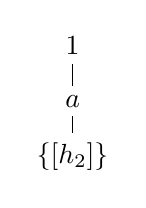
\begin{tikzpicture}[baseline={([yshift=-.5ex]current bounding box.center)},outer sep=auto, level distance=4em, scale=0.50]
    \node at (0, 0) {1}
      child {node {$a$}
        child {node {$\{[h_2]\}$}}};
  \end{tikzpicture}
  &&
  M_y\colon
  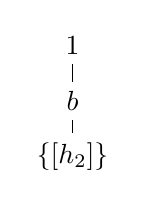
\begin{tikzpicture}[baseline={([yshift=-.5ex]current bounding box.center)},outer sep=auto, level distance=4em, scale=0.50]
    \node at (0, 0) {1}
      child {node {$b$}
        child {node {$\{[h_2]\}$}}};
  \end{tikzpicture}
\end{align*}

To find hypotheses compatible with $m$, we consider the set of variables $\vars(\lvl(m) + 1)$.
These are the variables shared between slot~$\lvl(m) + 1 = 2$ and all previous slots, i.e.\ $x$ and $y$.
Hence the compatible hypotheses are
\[
  \bigcap_{x \in \vars(\lvl(m) + 1)} H_{x}(i + 1, \sub(m)(x)) = H_{x}(2, a) \cap H_{y}(2, b) = \emptyset
\]
This means the match cannot currently be extended.
We now turn to the remaining hypothesis $h_3 : B~a~b$, adding it first to $H$.
This yields the following rule state:
\begin{align*}
  H_x\colon
  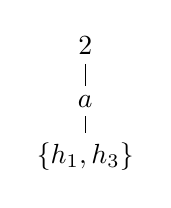
\begin{tikzpicture}[baseline={([yshift=-.5ex]current bounding box.center)},outer sep=auto, level distance=4em, scale=0.50]
    \node at (0, 0) {2}
      child {node {$a$}
        child {node {$\{h_1, h_3\}$}}};
  \end{tikzpicture}
  &&
  H_y\colon
  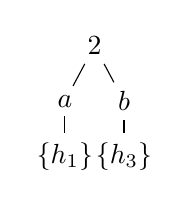
\begin{tikzpicture}[baseline={([yshift=-.5ex]current bounding box.center)},outer sep=auto, level distance=4em, scale=0.50]
    \node at (0, 0) {2}
      child {node {$a$}
        child {node {$\{h_1\}$}}}
      child {node {$b$}
        child {node {$\{h_3\}$}}};
  \end{tikzpicture}
  &&
  M_x\colon
  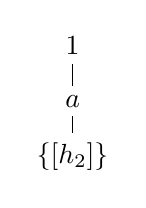
\begin{tikzpicture}[baseline={([yshift=-.5ex]current bounding box.center)},outer sep=auto, level distance=4em, scale=0.50]
    \node at (0, 0) {1}
      child {node {$a$}
        child {node {$\{[h_2]\}$}}};
  \end{tikzpicture}
  &&
  M_y\colon
  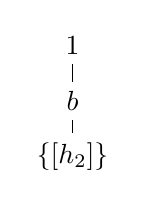
\begin{tikzpicture}[baseline={([yshift=-.5ex]current bounding box.center)},outer sep=auto, level distance=4em, scale=0.50]
    \node at (0, 0) {1}
      child {node {$b$}
        child {node {$\{[h_2]\}$}}};
  \end{tikzpicture}
\end{align*}
Since $h₃$ matches slot $i = 2$, the matches that can be extended by $h₃$ are
\[
  \bigcap_{x \in \vars(i)} M_{x}(i - 1, \sub_{i}(x)) = M_{x}(1, a) \cap M_{y}(1, b) = \{[h₂]\}
\]
This produces the complete match $[h₂, h₃]$, so we can add a new hypothesis of type $C~a~b$.

\section{Implementation}%
\label{sec:implementation}

Implementing the preceding technique efficiently requires some care, particularly in the context of dependent type theory.

\para{Matching.}
In type theory, types contain programs and matching (or, more generally, unification) is expected to respect definitional equality, i.e.\ equality up to evaluation.
For instance, a theorem with premise $P~2$, where $P$ is some predicate, should apply to a hypothesis of type $P~((\Lam{x}{x})~2)$ since the two types are definitionally equal.
As a result, matching premises and hypotheses is arbitrarily expensive in theory and a major cost centre in practice.
We therefore seek to avoid redundant invocations of the matching procedure.

To limit the cost of matching, we match with \emph{reducible transparency}.
Lean has multiple transparency levels that determine which constants are unfolded.
\enquote{Reducible} is the most restrictive of these, so we unfold few (and, in practice, only non-recursive) definitions.
Additionally, we use Lean's usual approximation of higher-order matching, which is complete for first-order matching problems and heuristically solves some higher-order problems.
Either of these limitations render forward reasoning incomplete, but since the same matching algorithm is used throughout Lean, users are used to this source of incompleteness.

\para{Normal Form.}
Since the hypothesis index $H$ and the match index $M$ of a rule state have the same domain, we combine them into one map.
This map, whose domain is a set of triples $(x, i, t)$, is represented by three nested persistent hash maps.

When looking up matching instantiations in the combined map, the instantiations should be compared up to definitional equality.
For example, the application of a theorem $\All{x}{P~x → Q~x → R~x}$ to hypotheses of type $P~a$ and $Q~((\Lam{x}{x})~a)$ should succeed even though $x$ is instantiated with different terms.
We therefore do not store $a$ and $(\Lam{x}{x})~a$ in the variable indices as is.
Instead, we bring all instantiations into \emph{reducible proof-irrelevant normal form} (RPINF).
This is the usual normal form of expressions with respect to Lean's notion of computation, with two modifications.
First, only \emph{reducible} defined constants are unfolded, reflecting our choice to perform unification at reducible transparency.
Second, parts of the original expression that are proofs (in the sense that their types are in the universe of propositions) are not normalised.
This is justified because Lean's type theory definitionally equates any two proofs of the same proposition, so there is no need to check whether they are equal.
When computing the RPINF, we also mark all proofs occurring in it with some special \enquote{metadata}.

With this setup, two expressions $t$ and $u$ are definitionally equal at reducible transparency if and only if their RPINFs are syntactically equal except for the marked proof subexpressions.
This notion of equality is syntactic, so it can be checked quickly and we can define an effective hash function that is compatible with it.
This allows us to use a hash map for the instantiations while still comparing them up to definitional equality.

There are reasons to believe that this scheme is more efficient than alternative schemes relying on repeated unifications.
For example, we could use Lean's discrimination trees, which implement a map from expressions to arbitrary data where lookup respects definitional equality.
However, these discrimination trees are imperfect, so the validity of a lookup result must be verified by matching the query expression against the expression that was originally stored in the discrimination tree.
We believe that this would generally be more expensive than calculating the RPINF of each hypothesis type (which can be cached).

\para{Match Equivalence.}
Naively, two matches would be considered equal if they contain the same hypotheses (up to definitional equality, again implemented via RPINF).
However, consider the rule $r : \All{x~y}{P~x~y → Q~x~z → R~x}$ and the hypotheses $h₁ : P~a~b$, $h₂ : P~a~c$, $h₃ : Q~a~d$ and $h₄ : Q~a~e$.
The complete matches $m₁ ≔ [h₁, h₃]$ and $m₁' ≔ [h₁, h₄]$ contain different hypotheses, but the difference does not matter because the applications $r~h₁~h₃$ and $r~h₁~h₄$ both have type $R~a$.
Generating both $m₁$ and $m₁'$ would therefore be redundant.
Similarly, the partial matches $m₂ ≔ [h₁]$ and $m₂' ≔ [h₂]$ are redundant because the choice between $h₁$ and $h₂$ affects neither the type of any eventual application derived from $m₂$ and $m₂'$ nor the hypotheses that can be used to complete them.
Hence we should store only one of $m₂$ and $m₂'$ in the rule state of $r$.
Based on these observations, we consider two matches $m$ and $m'$ of a rule $r$ with conclusion $A$ equal if $\lvl(m) = \lvl(m')$ and for each premise $x$ that appears either in the conclusion of $r$ or in the type of a slot $i$ of $r$ with $i > \lvl(m)$ we have $\sub(m)(x) = \sub(m')(x)$.

\para{Redundant Hypotheses.}
When we find a complete match, we add a new hypothesis of the corresponding type $T$ to the goal, but only if there is no other hypothesis of type $T$ already present.
To efficiently implement this check, we store in the forward state a set containing the RPINFs of all hypotheses that have been added to (and not subsequently removed from) the state.
We modified the naive forward reasoning implementation to use the same mechanism.

\para{Lazy Insertion.}
Adding a hypothesis to a rule state is cheap, but not free: it involves one unification for each slot that the hypothesis may match, according to a discrimination tree index, followed by several operations on the variable indices.
We therefore delay insertions until the index has selected at least one hypothesis for each slot.
This helps, for example, with the defining rule for involutive functions: if $f : α → α$ is involutive, then for any $a : α$ we have $f (f a) = a$.
When this rule is used as a forward rule, the premise $a$ matches any non-propositional hypothesis, but with lazy insertion we only process hypotheses for $a$ if there is, in fact, an involutive function in the context.

\section{Evaluation}%
\label{sec:evaluation}

There are unfortunately no standard benchmarks for Aesop-like tactics, and since Aesop is not expected to solve most goals without an extensive, manually curated set of rules, benchmarks for push-button theorem provers such as TPTP~\cite{TPTP} are not meaningful.
Additionally, forward rules are little used by Aesop's main client, the Mathlib library~\cite{Mathlib}.
We therefore only evaluate our technique against the previous, naive Aesop implementation on several synthetic benchmarks that demonstrate the performance characteristics of incremental forward reasoning.

For each benchmark, we set up certain forward rules and a goal with handpicked hypotheses.
We then run the \texttt{saturate} tactic, which uses either naive or incremental forward reasoning to exhaustively apply the forward rules.
Performing only forward reasoning is the best-case scenario for the incremental algorithm since previous results can be fully reused.
When forward reasoning is combined with other rules, we would expect smaller gains, depending on how much reuse the non-forward rules allow.

Instead of the natural number type of Lean's standard library, which has special support in the compiler and kernel, we use a custom type of Peano naturals for the benchmarks.
Matching two concrete Peano natural numbers $n$ and $m$ involves comparing $\min(n, m)$ constructors.
We can therefore use moderately large numbers to simulate the bigger matching problems that Aesop encounters, for example, in Mathlib's category theory development.

Benchmark code and data are available in our supplement~\cite{supplement}.
The results shown below were obtained on a MacBook Pro with an Apple~M2 Pro processor and \SI{32}{GB} of RAM, averaging over \textcolor{red}{N} (TODO) runs per benchmark.

\para{Transitivity Benchmark.}
Our first benchmark is a scaled-up variant of the transitivity example from Sec.~\ref{sec:incremental}.
Given some relation $≺$ on natural numbers, we register the lemma $\All{x~y}{x ≺ y → y ≺ z → x ≺ z}$ as the sole forward rule and set up a goal with hypotheses $h₁ : a ≺ a + 1, \dots, hₙ : a + n - 1 ≺ a + n$, where either $a = 0$ (yielding easy unification problems) or $a = 100$.
Saturating this goal adds $n(n-1)/2$ hypotheses to the context.

\begin{figure}
  \centering
  \begin{subfigure}[b]{.5\textwidth}
    \centering
    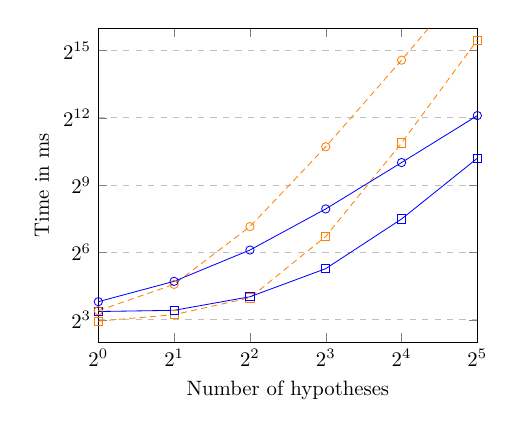
\begin{tikzpicture}[scale=0.75]
      \begin{axis}[
        xlabel={Number of hypotheses},
        ylabel={Time in ms},
        xmin=1, xmax=32,
        ymin=4, ymax=2^16,
        %xtick={1,2,4,8,16},
        %ytick={2^3,2^5,2^7,2^9,2^11,2^13},
        xmode=log,
        ymode=log,
        log basis x=2,
        log basis y=2,
        legend pos=north west,
        ymajorgrids=true,
        grid style=dashed,
        legend image post style={mark=}
        ]
        \addplot[
          color=orange,
          mark=square,
          style=densely dashed,
          mark options={style={solid}}
          ]
          coordinates {
            (1, 7.663472) (2, 9.354750) (4, 15.768194) (8, 104.921791) (16, 1882.683111) (32, 45220.919667)  
          };
        \addplot[
          color=blue,
          mark=square,
          ]
          coordinates {
            (1, 10.308541) (2, 10.704638) (4, 16.274305) (8, 38.800833) (16, 179.697681) (32, 1175.888750)
          };
        \addplot[
          color=orange,
          mark=o,
          style=densely dashed,
          mark options={style={solid}}
          ]
          coordinates {
            (1, 10.591138) (2, 23.881333) (4, 142.013389) (8, 1676.148375) (16, 24327.359417) (32, 392049.849708) 
          };
        \addplot[
          color=blue,
          mark=o,
          ]
          coordinates {
            (1, 13.974694) (2, 26.216833) (4, 68.953444) (8, 245.601028) (16, 1028.670680) (32, 4388.917500) 
          };
      \end{axis}
    \end{tikzpicture}
    \caption{Transitivity benchmark}%
    \label{fig:trans}
  \end{subfigure}%
  \begin{subfigure}[b]{.5\textwidth}
    \centering
    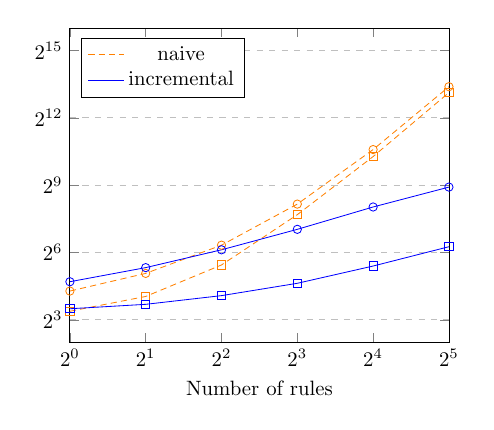
\begin{tikzpicture}[scale=0.75]
      \begin{axis}[
        xlabel={Number of rules},
        %ylabel={Time in ms},
        xmin=1, xmax=32,
        ymin=4, ymax=2^16,
        ymode=log,xmode=log,
        log basis x=2,
        log basis y=2,
        legend pos=north west,
        ymajorgrids=true,
        grid style=dashed,
        legend image post style={mark=},
        ]
        \addplot[
          color=orange,
          mark=square,
          style=densely dashed,
          mark options={style={solid}}
          ]
          coordinates {
            (1, 10.399958) (2, 16.426541) (4, 43.461403) (8, 205.595541) (16, 1238.090889) (32, 8927.857819)
          };
          \addlegendentry{naive}
        \addplot[
          color=blue,
          mark=square,
          ]
          coordinates {
            (1, 11.231875) (2, 12.879500) (4, 16.851930) (8, 24.666485) (16, 42.054055) (32, 76.369778)
          };
          \addlegendentry{incremental}
        \addplot[
          color=orange,
          mark=o,
          style=densely dashed,
          mark options={style={solid}}
          ]
          coordinates {
            (1, 19.405222) (2, 33.487472) (4, 80.107597) (8, 284.954791) (16, 1536.089624) (32, 10721.729861)
          };
        \addplot[
          color=blue,
          mark=o,
          ]
          coordinates {
            (1, 25.892069) (2, 40.031930) (4, 69.446902) (8, 130.640986) (16, 260.653917) (32, 481.827902)
          };
      \end{axis}
    \end{tikzpicture}
    \caption{Independence benchmark}%
    \label{fig:indep}
  \end{subfigure}
  \caption{Results of the transitivity (\subref{fig:trans}) and independence (\subref{fig:indep}) benchmarks for $a = 0$ (\protect\showpgfsquare) and $a = 100$ (\protect\showpgfcircle).}%
  \label{fig:benchmark}
  \end{figure}

Fig.~\ref{fig:trans} shows that the incremental algorithm has a sizeable advantage over the naive algorithm.
The scales are logarithmic, with each dotted horizontal line representing an 8-fold increase.
Hence, for $2^{5} = 32$ hypotheses and $a = 0$, incremental forward reasoning is over 38 times faster than naive forward reasoning.
The difference for $a = 100$ is even larger.

These results are unsurprising, given the complexity of both algorithms on this benchmark.
The naive algorithm goes over the context, containing initially $n$ hypotheses, and compares all hypotheses pairwise.
This is repeated approximately for each of the $n(n-1)/2$ added hypotheses, so the overall complexity is $O(n^4)$.
By contrast, the incremental algorithm considers each hypothesis only once, matching it against both slots and then comparing it with at most $n$ other hypotheses, so the complexity is $O(n^{2})$.

Both algorithms generate all possible transitivity chains.
If only the longest such chain, from $a$ to $a + n$, is desired, the transitivity rule can be registered as a \emph{destruct} rule, a special sort of forward rule that removes from the context any hypotheses it is applied to.
This reduces the complexity of the incremental algorithm to $O(n)$.

\para{Independence Benchmark.}
In the previous example, the incremental algorithm performs well partly because each match at level~1 can be combined with many hypotheses at level~2 without processing the level~1 hypothesis repeatedly.
We now consider a benchmark with many independent rules where this kind of reuse does not occur.

Given $n ≥ 1$, we use $n$ forward rules of the form $\All{x}{P_{1}~x → \dots → P_{6}~x → Q~x}$, where $P_{1}, \dots, P_{6}$ and $Q$ are arbitrary predicates that are distinct from each other and from the predicates of all other rules.
The initial goal contains one hypothesis of type $P_{i}~a$ for each predicate $P_{i}$ that appears in a rule slot, where $a$ is again either 0 or 100.
Hence, each rule can be applied exactly once and each hypothesis matches exactly one slot.

Still, Fig.~\ref{fig:indep} shows that the incremental approach outperforms the naive one for $n ≥ 4$.
This is because incrementality helps even in this scenario.
Whenever a hypothesis is added (and hence a new subgoal created), the naive algorithm re-runs all the rules it had already run on the previous subgoal, realising only after the fact that the rules were already applied.
The incremental algorithm avoids this source of redundancy.
Accordingly, the naive algorithm has complexity $O(n^{3})$ on this benchmark, versus $O(n)$ for the incremental algorithm.

\begin{figure}
  \centering
  \begin{subfigure}{.5\textwidth}
    \centering
    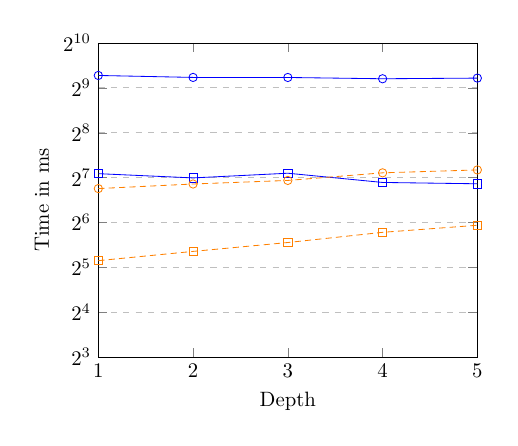
\begin{tikzpicture}[scale=0.75]
      \begin{axis}[
        xlabel={Depth},
        ylabel={Time in ms},
        xmin=1, xmax=5,
        ymin=8, ymax=2^10,
        xtick={1,2,3,4,5},
        ymode=log,
        log basis y=2,
        ymajorgrids=true,
        grid style=dashed
        ]
        \addplot[
          color=orange,
          mark=square,
          style=densely dashed,
          mark options={style={solid}}
          ]
          coordinates {
            (1, 35.466292) (2, 40.918638) (3, 46.936125) (4, 54.933124) (5, 61.269861)
          };
        \addplot[
          color=blue,
          mark=square,
          ]
          coordinates {
            (1, 135.967736) (2, 127.324444) (3, 136.891250) (4, 118.720444) (5, 116.293222)
          };
        \addplot[
          color=orange,
          mark=o,
          style=densely dashed,
          mark options={style={solid}}
          ]
          coordinates {
            (1, 107.978069) (2, 115.900527) (3, 122.454958) (4, 137.732764) (5, 144.037681)
          };
        \addplot[
          color=blue,
          mark=o,
          ]
          coordinates {
            (1, 619.932611) (2, 601.456805) (3, 600.926110) (4, 589.144389) (5, 595.091180)
          };
      \end{axis}
    \end{tikzpicture}
    \caption{Without precompilation}%
    \label{fig:erase-noprecomp}
  \end{subfigure}%
  \begin{subfigure}{.5\textwidth}
    \centering
    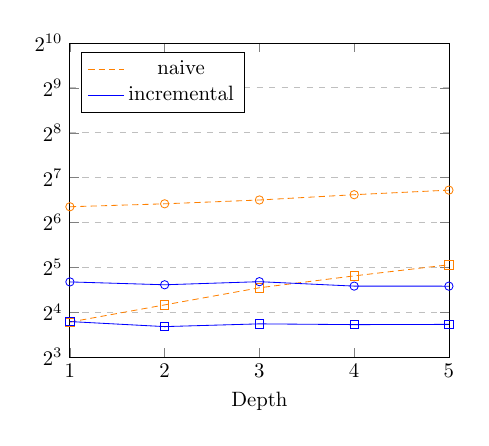
\begin{tikzpicture}[scale=0.75]
      \begin{axis}[
        xlabel={Depth},
        xmin=1, xmax=5,
        ymin=8, ymax=1024,
        xtick={1,2,3,4,5},
        ymode=log,
        log basis y=2,
        %yticklabels={},
        legend pos=north west,
        ymajorgrids=true,
        grid style=dashed,
        legend image post style={mark=},
        ]
        \addplot[
          color=orange,
          mark=square,
          style=densely dashed,
          mark options={style={solid}}
          ]
          coordinates {
            (1, 13.728805) (2, 17.909194) (3, 23.324666) (4, 28.030819) (5, 33.279611)
          };
        \addlegendentry{naive}
        \addplot[
          color=blue,
          mark=square,
          ]
          coordinates {
            (1, 13.841305) (2, 12.801791) (3, 13.358389) (4, 13.200611) (5, 13.251902)
          };
        \addlegendentry{incremental}
        \addplot[
          color=orange,
          mark=o,
          style=densely dashed,
          mark options={style={solid}}
          ]
          coordinates {
            (1, 81.546486) (2, 85.345444) (3, 90.532347) (4, 98.247764) (5, 105.423875)
          };
        \addplot[
          color=blue,
          mark=o,
          ]
          coordinates {
            (1, 25.539097) (2, 24.432485) (3, 25.629666) (4, 23.935250) (5, 23.911139)
          };
      \end{axis}
    \end{tikzpicture}
    \caption{With precompilation}%
    \label{fig:erase-precomp}
  \end{subfigure}
  \caption{Results of the depth benchmark for $n = 6$ with precompilation disabled (\subref{fig:erase-noprecomp}) or enabled (\subref{fig:erase-precomp}) and with $a = 0$ (\protect\showpgfsquare) or $a = 100$ (\protect\showpgfcircle).}%
  \label{fig:erase}
\end{figure}

\para{Depth Benchmark.}
Our final benchmark concerns situations where many rules match almost, but not quite.
We use 100 copies of a rule $r : \All{x}{P_{1}~x → \dots → P_{n}~x → A}$, where the predicates $P_{i}$ are all distinct and $A$ is an arbitrary proposition.
Given a \emph{depth} $k ≤ n$, the initial goal contains hypotheses of types $P_{i}~a$ for each $i ≠ n - k$ with $1 ≤ i ≤ n$, as well as one hypothesis $P_{n-k}~(a + 1)$ (with $a = 0$ or $a = 100$).
In other words, the hypotheses match all premises with compatible substitutions, except the $k$th premise from the back.
Since the naive algorithm processes the premises from back to front, $k$ determines how many premises the algorithm matches before it notices that the rule cannot be applied.

This setup is challenging for the incremental algorithm because (1) no rule is ever applied, so incrementality does not help; and (2) the incremental algorithm expends a non-negligible amount of effort for each of the $n$ hypotheses, whereas the naive algorithm can, at least for small $k$, decide fairly quickly that the rule is not applicable.
And indeed, Fig.~\ref{fig:erase-noprecomp} shows that while the naive approach slows down for greater $k$ (though not by much since the context contains only $n = 6$ hypotheses), big constant factors cause the incremental approach to remain slower for $k$ up to 5.

Fig.~\ref{fig:erase-precomp}, however, shows a different picture, with the incremental approach leading for all $k > 1$.
The figure visualises the results of the depth benchmark with \emph{precompilation} enabled.
This is a feature of Lean that compiles tactics ahead of time instead of interpreting them.
Our technique appears to benefit from this much more than the naive approach, perhaps because the RPINF calculation incurs a large interpretation overhead.
We observe the same effect when enabling precompilation for the other benchmarks.
Unfortunately, precompilation also substantially increases Aesop's build time and slows down Lean's build tool, Lake, so we disable it by default, but users of Aesop can choose to enable it for faster forward reasoning.

\section{Related Work}

\para{White-Box Tactics.}
Among white-box proof automation tactics, to our knowledge only ACL2's \enquote{waterfall}~\cite{ACL2} and PVS's various proof search strategies~\cite{PVS} have special support for forward reasoning.
Both use techniques similar to Aesop's naive algorithm; in particular, the context of each goal is saturated independently.
ACL2 additionally allows forward rules to be annotated with \emph{trigger terms}, which cause the rules to be run if the trigger terms are matched anywhere in a goal.
Aesop implements a similar mechanism, \emph{rule patterns}, not described here due to space constraints.

The auto2 tactic~\cite{auto2} employs an SMT-like search procedure based on forward reasoning and e-matching~\cite{simplify}.
As such, it does not require incrementality, but it could perhaps benefit from indexing along the lines of our variable indices.

\para{SATCHMO.}
The SATCHMO first-order theorem prover~\cite{SATCHMO} uses a search procedure that treats a given set of implications as forward rules and uses a case-splitting rule to perform case analysis on disjunctive hypotheses.
SATCHMO-style provers may benefit from our incremental approach if the set of implications is large.
However, since unification is comparatively cheap in first-order logic, it is not clear whether avoiding repeated unifications outweighs the cost of maintaining the forward state.
SATCHMO also employs an optimisation that \enquote*{focuses} forward reasoning on the hypothesis established by the last case split, providing a different form of incrementality.

\para{Knowledge-Based Systems.}
Some knowledge-based reasoning systems, e.g.\ Algernon~\cite{Algernon} and EYE~\cite{EYE}, support combined forward and backward reasoning.
However, to our knowledge, no such system allows non-forward rules to change the assumptions available to forward rules, so they do not require incrementality.
Nevertheless, our technique bears some resemblance to the RETE algorithm~\cite{RETE} for forward reasoning in large knowledge bases.

\section{Conclusion}

We have presented a technique that integrates forward reasoning into a tree-based proof search procedure supporting arbitrary proof rules.
We avoid redundant reasoning steps by caching partial forward rule applications in a data structure, the \emph{forward state}, that enables efficient updates.
The technique is independent of the search strategy and logic used.
Our evaluation shows substantial speedups on synthetic benchmarks, relative to Aesop's previous implementation.

One obvious extension of our method would be to exploit redundancy not just between contexts of parent and child goals, but also between those of siblings or even unrelated goals.
The forward state supports this since for any two goals, we can adapt a goal's saved forward state to a similar goal.

\para{Acknowledgements.}
We thank Jasmin Blanchette and Massin Guerdi for their valuable comments on drafts of this paper.
Généreux's research was co-funded by the European Union (ERC, Nekoka, 101083038) and by the Fonds de recherche du Québec, 330205. Views and opinions expressed are however those of the authors only and do not necessarily reflect those of the European Union or the European Research Council. Neither the European Union nor the granting authority can be held responsible for them.

\bibliography{lit}

\end{document}
